% In-situ JES: storage floor, jet-cut, JER-extrapolation and timing variations (Oct 7-8, 2026)
\documentclass[aspectratio=169,10pt]{beamer}
\usepackage[T1]{fontenc}
\usepackage[utf8]{inputenc}
\usepackage{booktabs}
\usepackage{graphicx}
\usepackage{amsmath}
\setbeamertemplate{navigation symbols}{}
\setbeamertemplate{footline}{\hfill\insertframenumber\,/\,\inserttotalframenumber\hspace{1em}\vspace{0.6em}}
\newcommand{\pa}{p_{a}}
\newcommand{\xjg}{x_{J\gamma}}

\title{In-situ JES: cut, timing and JER-smearing variations}
\subtitle{$\gamma$+jet, p+p Run 24 data and Pythia8}
\author{Samuel F.\ Liechty}
\date{October 8, 2026}

\begin{document}

\begin{frame}
  \titlepage
\end{frame}

% ------------------------------------------------------------------
\begin{frame}{Nominal in-situ JES (5 GeV jet cut)}
  \begin{columns}[T]
    \begin{column}{0.52\textwidth}
      \footnotesize
      \begin{tabular}{lcccc}
        \toprule
        R & $\pa$ & stat $-/+$ & syst $-/+$ & previous \\
        \midrule
        0.2 & 0.9013 & 0.0081 / 0.0085 & 0.103 / 0.103 & 0.9034 \\
        0.3 & 0.9001 & 0.0047 / 0.0049 & 0.008 / 0.021 & 0.9158 \\
        0.4 & 0.9101 & 0.0082 / 0.0061 & 0.015 / 0.016 & 0.9265 \\
        0.5 & 0.9064 & 0.0060 / 0.0078 & 0.015 / 0.022 & 0.9259 \\
        0.6 & 0.9123 & 0.0064 / 0.0081 & 0.010 / 0.018 & 0.9292 \\
        0.7 & 0.9072 & 0.0078 / 0.0081 & 0.011 / 0.017 & 0.9295 \\
        0.8 & 0.9220 & 0.0072 / 0.0077 & 0.014 / 0.020 & 0.9519 \\
        \bottomrule
      \end{tabular}
      \vspace{0.6em}
      \begin{itemize}
        \item Full pipeline on the Oct 5 trees; converged after 3 scans (last change 0.0005).
        \item ``Previous'' is the table from the older trees.
        \item R = 0.2 syst.\ is set by the three-jet variation, which sits at the scan edge (0.800).
      \end{itemize}
    \end{column}
    \begin{column}{0.46\textwidth}
      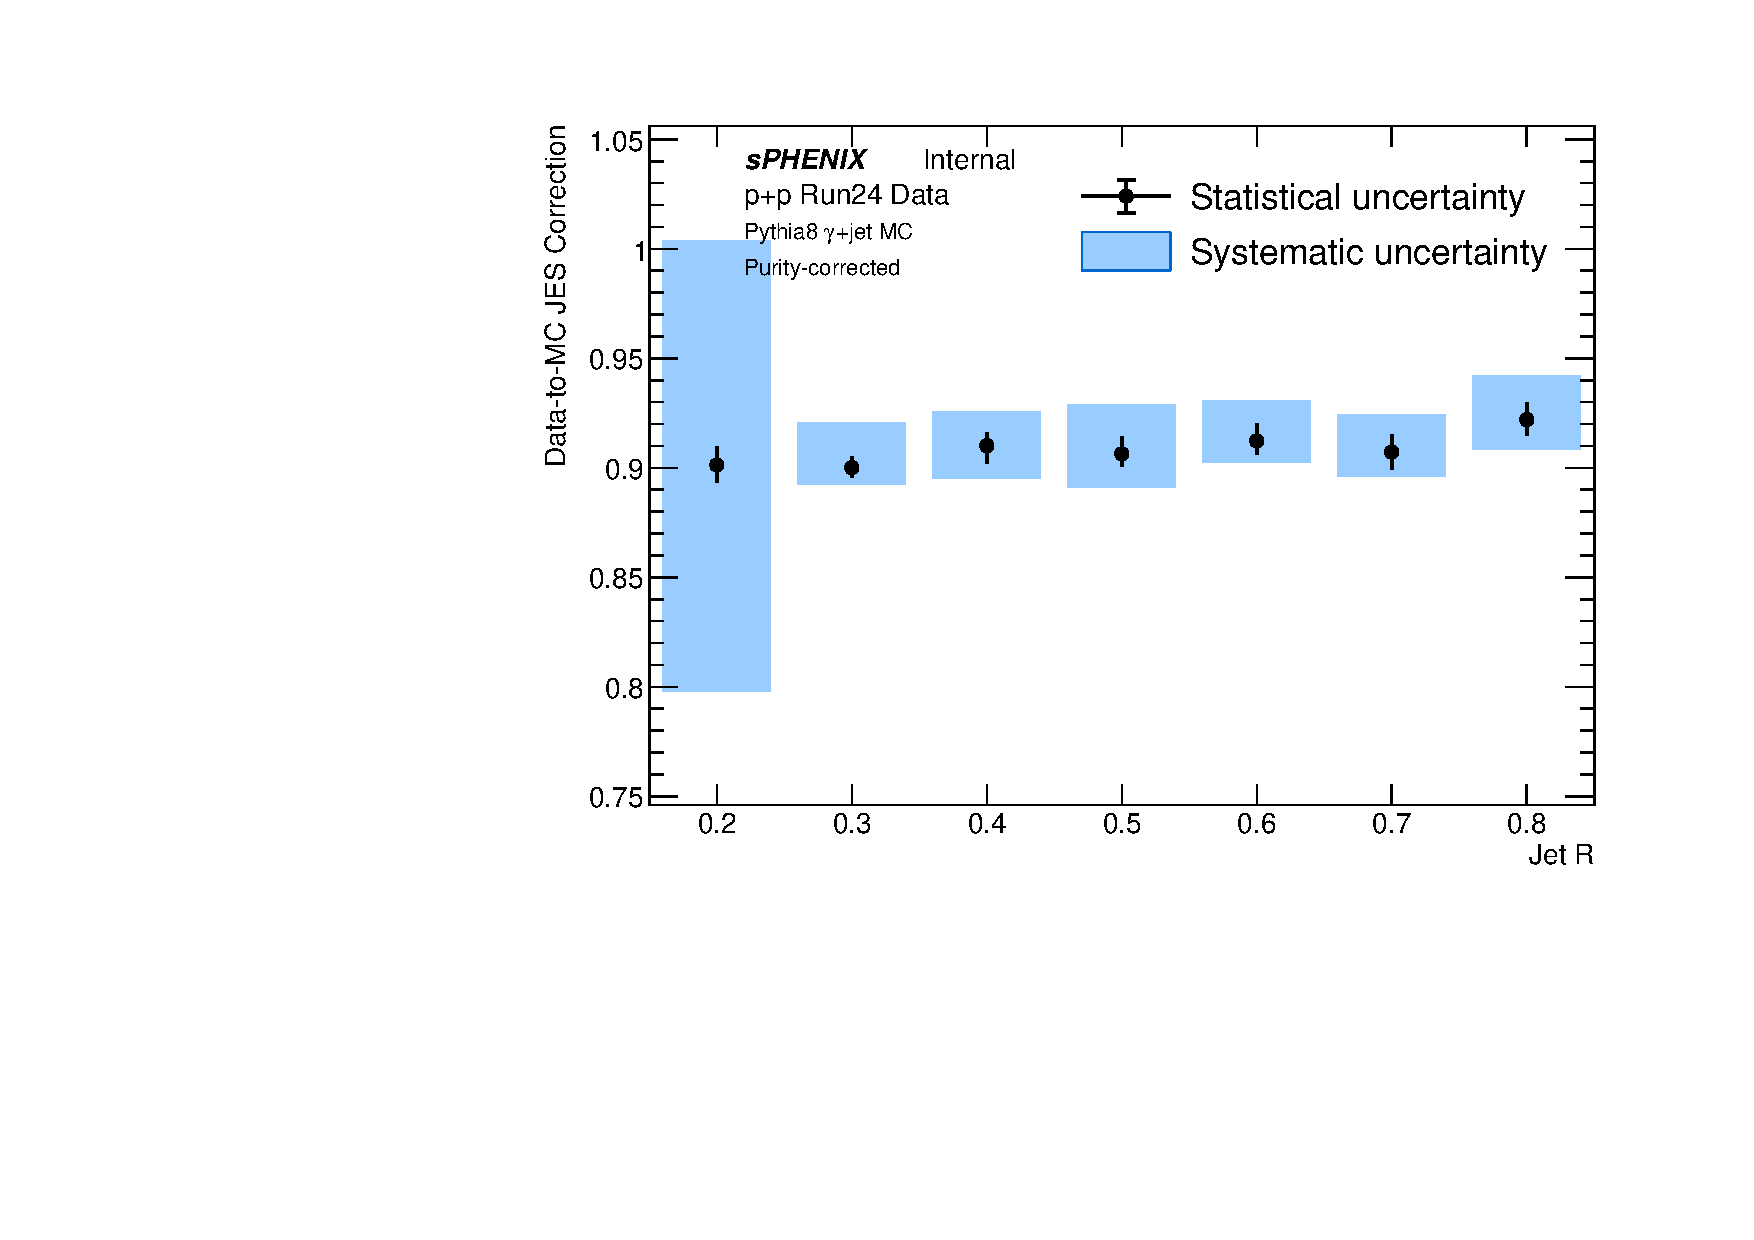
\includegraphics[width=\linewidth]{figs/jes_summary_nominal.pdf}
    \end{column}
  \end{columns}
\end{frame}

% ------------------------------------------------------------------
\begin{frame}{Which jets are stored in the $\gamma$+jet trees}
  \begin{columns}[T]
    \begin{column}{0.5\textwidth}
      \small
      A jet is stored if any of these holds (\texttt{CaloAna.cc}):
      \begin{itemize}
        \item raw $p_T \geq 3$ GeV;
        \item calibrated $p_T \geq 5$ GeV, or calibrated / 0.90 $\geq 5$ GeV;
        \item MC: any of the six smeared $p_T$ values $\geq 5$ GeV.
      \end{itemize}
      \vspace{0.5em}
      \begin{itemize}
        \item Data: complete from calibrated 4.5 GeV. At 4.0--4.5 GeV only $\sim$20\% are stored.
        \item MC: the stored third-jet $p_T$ (truth-anchored smear) is complete from 5.0 GeV.
      \end{itemize}
    \end{column}
    \begin{column}{0.48\textwidth}
      \small
      Third-jet $p_T$, R = 0.4, entries per 0.25 GeV:
      \vspace{0.3em}

      \centering
      \begin{tabular}{lcc}
        \toprule
        $p_T$ (GeV) & Data & Pythia Photon10 \\
        \midrule
        3.75 & 23 & 40806 \\
        4.00 & 7860 & 41142 \\
        4.25 & 8973 & 41704 \\
        4.50 & 39860 & 41617 \\
        4.75 & 34049 & 41637 \\
        5.00 & 29493 & 68541 \\
        5.25 & 24796 & 63922 \\
        \bottomrule
      \end{tabular}
    \end{column}
  \end{columns}
\end{frame}

% ------------------------------------------------------------------
\begin{frame}{What the storage floor affects}
  \small
  \textbf{Three-jet veto:} data third jet $> 5\text{ GeV} \times \pa$, with no $\xjg$ floor.
  \begin{itemize}
    \item At $\pa = 0.80$ the veto is at 4.0 GeV, in the incomplete region, so data is under-vetoed.
    \item This is the variation that runs to the scan edge at R = 0.2.
  \end{itemize}
  \vspace{0.5em}
  \textbf{Recoil jet:} the scan applies the $\xjg$ floor after dividing by $\pa$.
  \vspace{0.3em}

  \centering
  \begin{tabular}{lcc}
    \toprule
    photon $p_T$ & $\xjg$ floor & softest calibrated jet used \\
    \midrule
    15--20 GeV & 0.40 & $6.0 \times \pa$ \\
    20--25 GeV & 0.30 & $6.0 \times \pa$ \\
    25--35 GeV & 0.30 & $7.5 \times \pa$ \\
    \bottomrule
  \end{tabular}
  \vspace{0.3em}
  \begin{itemize}
    \item At the scan edge ($\pa = 0.80$) that is 4.8 GeV, above the 4.5 GeV completeness.
    \item The nominal $\pa$ is not at a floor.
  \end{itemize}
  \vspace{0.3em}
  \raggedright
  Treemaker fix (built on SDCC, needs a reprocess): store jets down to 4.0 GeV and add \texttt{thirdjet\_pt\_calib}.
\end{frame}

% ------------------------------------------------------------------
\begin{frame}{Jet $p_T$ cut: 5, 7 and 9 GeV}
  \small
  Recoil-jet cut and three-jet veto changed together. 7 and 9 GeV: one scan, starting from the converged 5 GeV table.
  \vspace{0.5em}

  \centering
  \begin{tabular}{lccccccc}
    \toprule
    R & 0.2 & 0.3 & 0.4 & 0.5 & 0.6 & 0.7 & 0.8 \\
    \midrule
    5 GeV (nominal) & 0.9013 & 0.9001 & 0.9101 & 0.9064 & 0.9123 & 0.9072 & 0.9220 \\
    7 GeV & 0.8986 & 0.9070 & 0.9115 & 0.9140 & 0.9111 & 0.9067 & 0.9183 \\
    9 GeV & 0.8895 & 0.9146 & 0.9168 & 0.9137 & 0.9047 & 0.8994 & 0.9127 \\
    \midrule
    7 -- 5 GeV & $-0.003$ & $+0.007$ & $+0.001$ & $+0.008$ & $-0.001$ & $-0.000$ & $-0.004$ \\
    9 -- 5 GeV & $-0.012$ & $+0.015$ & $+0.007$ & $+0.007$ & $-0.008$ & $-0.008$ & $-0.009$ \\
    \bottomrule
  \end{tabular}
  \vspace{0.6em}
  \raggedright
  \begin{itemize}
    \item 7 GeV agrees with 5 GeV within 1\% at every R.
    \item 9 GeV moves R = 0.2 by $-1.3$\% and R = 0.3 by $+1.7$\%.
    \item The three-jet variation at R = 0.2 is off the scan edge: 0.9055 (7 GeV), 0.8982 (9 GeV).
  \end{itemize}
\end{frame}

% ------------------------------------------------------------------
\begin{frame}{JER smearing width below its measured range}
  \begin{columns}[T]
    \begin{column}{0.5\textwidth}
      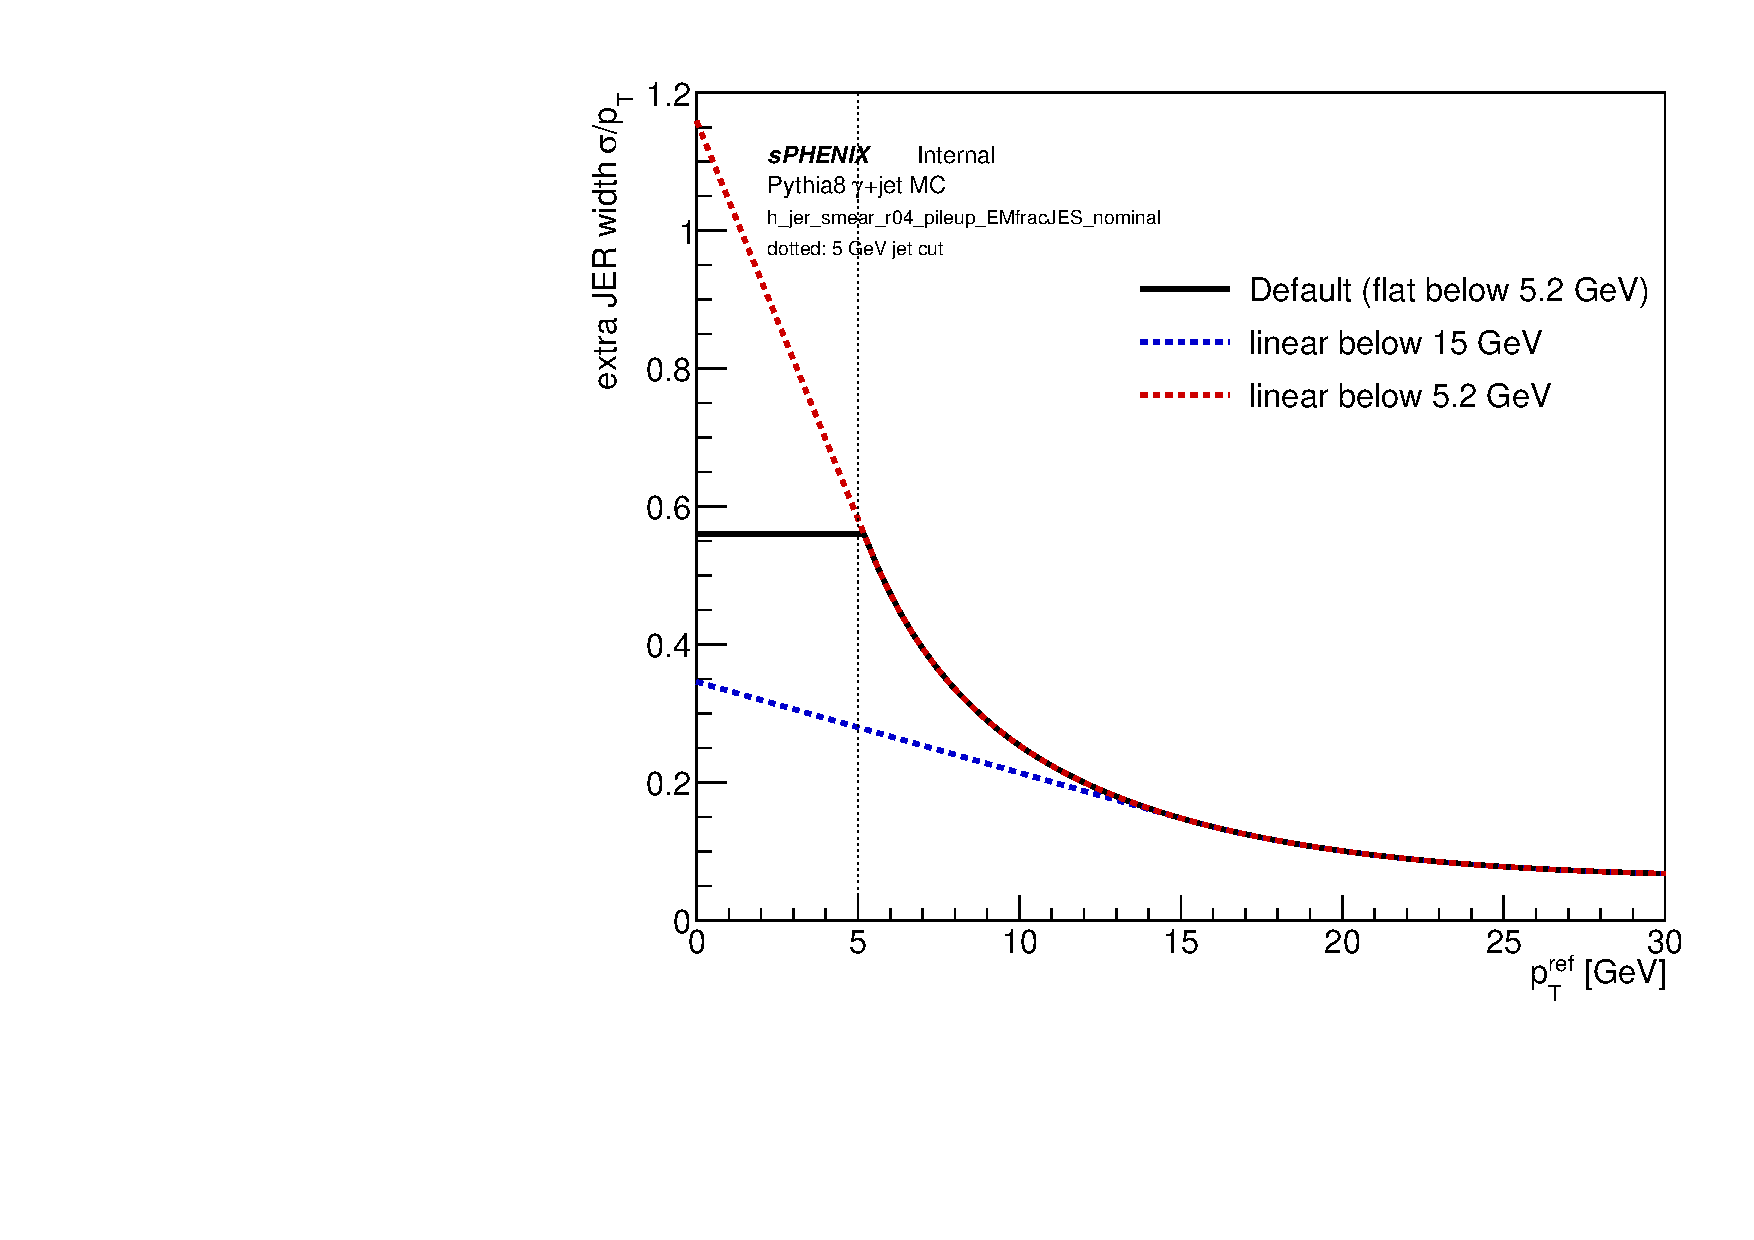
\includegraphics[width=\linewidth,page=1]{figs/jer_extrap.pdf}
    \end{column}
    \begin{column}{0.48\textwidth}
      \small
      \begin{itemize}
        \item Default: the template, flat below 5.2 GeV.
        \item Linear below 15 GeV: its tangent at 15 GeV.
        \item Linear below 5.2 GeV: its first segment.
      \end{itemize}
      \vspace{0.4em}
      Method (MC, nominal width only):
      \begin{itemize}
        \item Smear deviate recovered from the stored smeared $p_T$, then reused with the new width.
        \item Reference $p_T$: calibrated $p_T$ below 5 GeV (exact), else the truth recoil jet within $0.75R$, else calibrated $p_T$.
        \item Region-A R = 0.4 pairs: 1.2\% exact, 93.0\% truth-matched, 5.8\% fallback.
      \end{itemize}
    \end{column}
  \end{columns}
\end{frame}

% ------------------------------------------------------------------
\begin{frame}{JER extrapolation: MC $\xjg$, R = 0.4, region A}
  \centering
  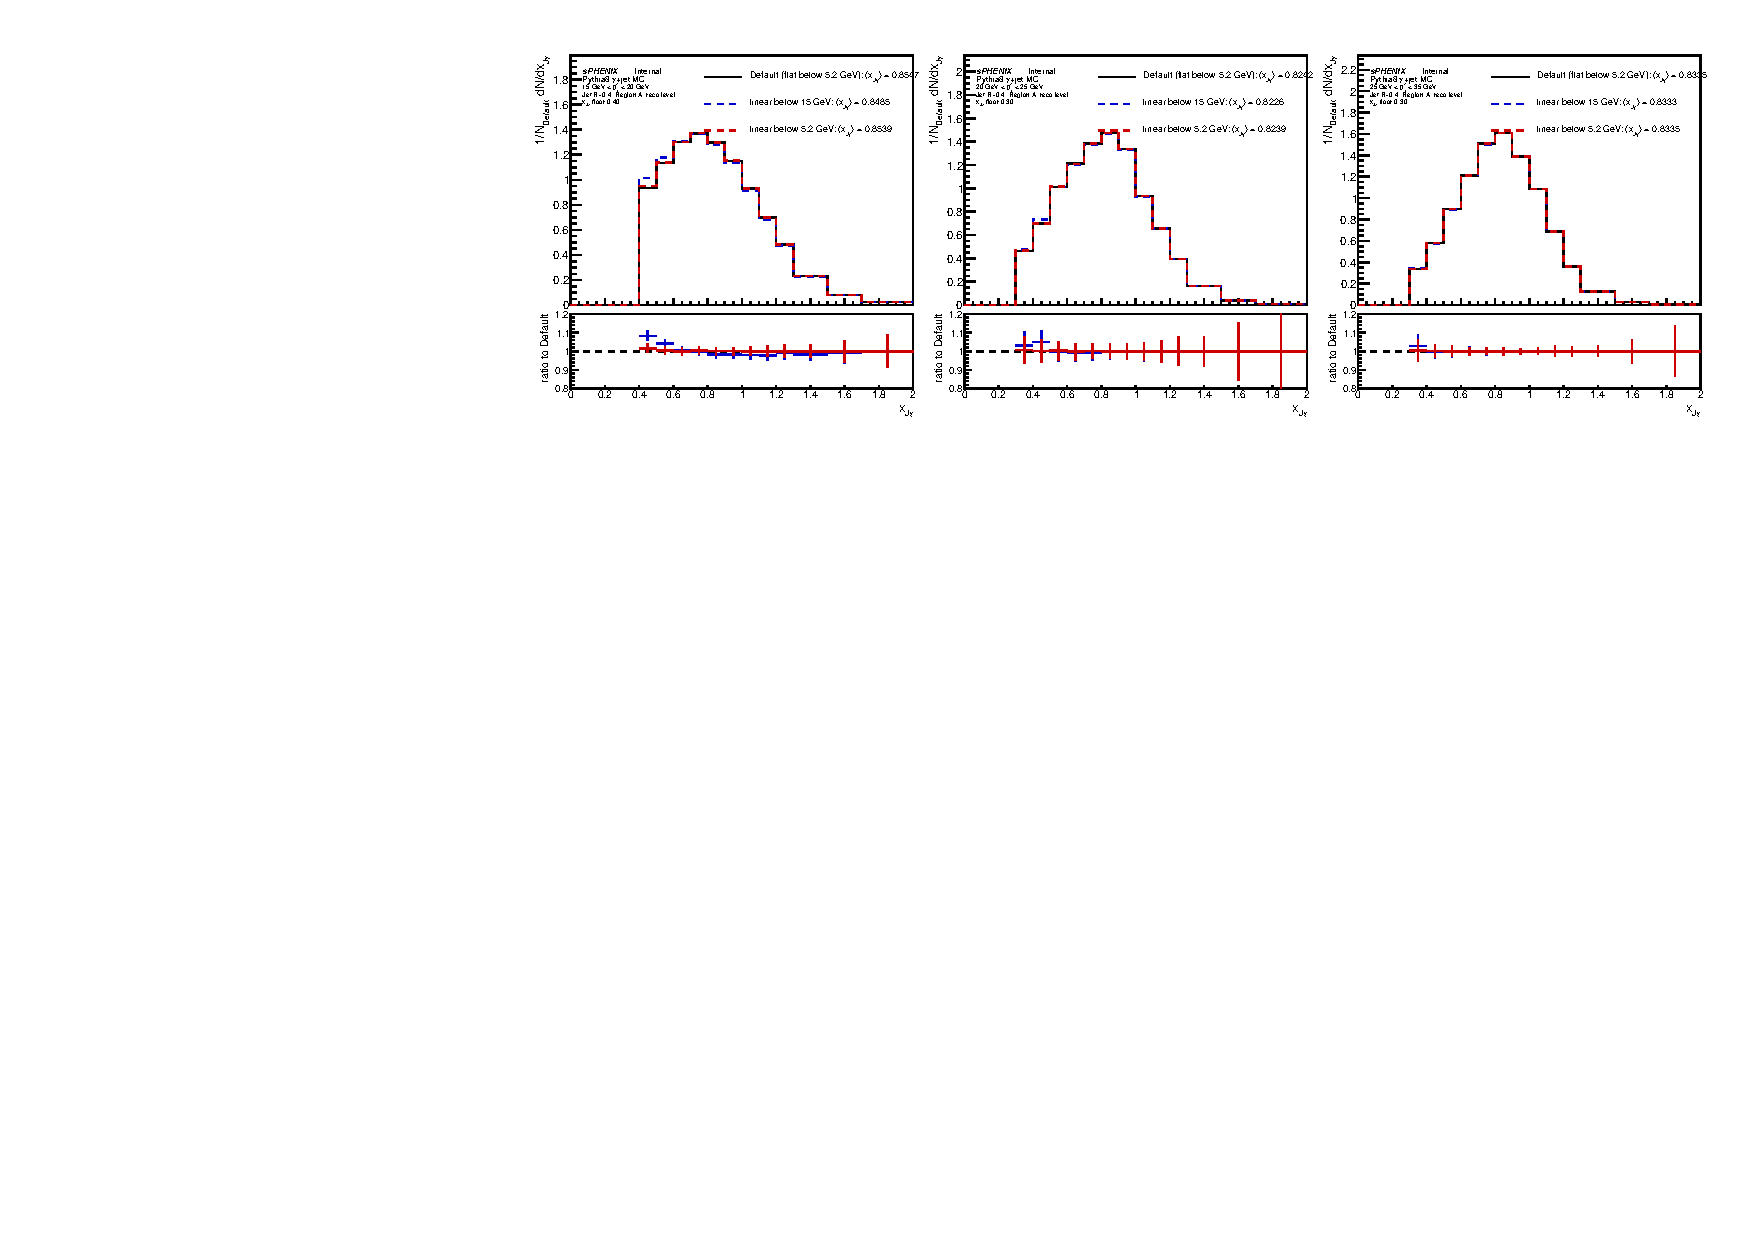
\includegraphics[width=\linewidth]{figs/jer_extrap_xj.pdf}
  \vspace{0.3em}

  \small
  \raggedright
  \begin{itemize}
    \item All curves scaled by the Default histogram's integral; ratios to Default below.
    \item Linear below 15 GeV differs mainly at low $\xjg$ in the 15--20 GeV bin.
  \end{itemize}
\end{frame}

% ------------------------------------------------------------------
\begin{frame}{JER extrapolation: MC reference and in-situ $\pa$}
  \begin{columns}[T]
    \begin{column}{0.48\textwidth}
      \centering\includegraphics[height=0.6\textheight,page=4]{figs/jer_extrap.pdf}
    \end{column}
    \begin{column}{0.48\textwidth}
      \centering\includegraphics[height=0.6\textheight,page=5]{figs/jer_extrap.pdf}
    \end{column}
  \end{columns}
  \footnotesize
  \centering
  \begin{tabular}{lccccccc}
    \toprule
    $\Delta\pa$ vs Default & 0.2 & 0.3 & 0.4 & 0.5 & 0.6 & 0.7 & 0.8 \\
    \midrule
    linear below 15 GeV & $+0.013$ & $+0.010$ & $+0.005$ & $+0.005$ & $+0.005$ & $+0.002$ & $+0.001$ \\
    linear below 5.2 GeV & $+0.002$ & $+0.003$ & $0.000$ & $+0.001$ & $0.000$ & $+0.001$ & $0.000$ \\
    \bottomrule
  \end{tabular}
\end{frame}

% ------------------------------------------------------------------
\begin{frame}{Timing, R = 0.4: object time relative to the MBD}
  \begin{columns}[T]
    \begin{column}{0.6\textwidth}
      \includegraphics[width=\linewidth,page=3]{figs/timing_r04.pdf}

      \includegraphics[width=\linewidth,page=4]{figs/timing_r04.pdf}
    \end{column}
    \begin{column}{0.38\textwidth}
      \footnotesize
      Region-A pairs in data, 15--35 GeV, 3729 pairs.
      \vspace{0.3em}

      \begin{tabular}{lcc}
        \toprule
        (ns) & mean & RMS \\
        \midrule
        $t_{cl}$ & $-2.18$ & 2.40 \\
        $t_{jet}$ & $-1.65$ & 2.16 \\
        $t_{cl} - t_{MBD}$ & $-1.99$ & 0.67 \\
        $t_{jet} - t_{MBD}$ & $-1.46$ & 1.18 \\
        $t_{cl} - t_{jet}$ & $-0.53$ & 1.12 \\
        \bottomrule
      \end{tabular}
      \vspace{0.4em}
      \begin{itemize}
        \item Treemaking windows (dashed): cluster $-4$ to 0 ns, jet $-5$ to 2 ns.
        \item Stored objects are inside them.
      \end{itemize}
    \end{column}
  \end{columns}
\end{frame}

% ------------------------------------------------------------------
\begin{frame}{Timing, R = 0.4: dependence on jet $p_T$}
  \begin{columns}[T]
    \begin{column}{0.6\textwidth}
      \includegraphics[width=\linewidth,page=9]{figs/timing_r04.pdf}

      \includegraphics[width=\linewidth,page=11]{figs/timing_r04.pdf}
    \end{column}
    \begin{column}{0.38\textwidth}
      \small
      Mean per bin (red):
      \begin{itemize}
        \item $t_{jet} - t_{MBD}$: $-1.08$ ns at 5--8 GeV, $-1.84$ ns at 24--35 GeV.
        \item $t_{cl} - t_{jet}$: $-0.95$ ns at 5--8 GeV, $-0.14$ to $-0.17$ ns at 24--35 GeV.
        \item $t_{cl} - t_{MBD}$ vs photon $p_T$: flat at $\sim -2.0$ ns from 15 to 27 GeV.
      \end{itemize}
    \end{column}
  \end{columns}
\end{frame}

% ------------------------------------------------------------------
\begin{frame}{Multijet timing cut vs $\gamma$+jet}
  \small
  \begin{columns}[T]
    \begin{column}{0.48\textwidth}
      \textbf{Multijet} (data, whole event dropped):
      \begin{itemize}
        \item Skim: $|t_{lead} + 2| < 6$ ns and $|t_{lead} - t_{sub}| < 3$ ns.
        \item Analysis: the same on \texttt{corrMaxJett}/\texttt{corrSubJett}, centred at 0.
      \end{itemize}
      \textbf{$\gamma$+jet} (data, per object, relative to MBD):
      \begin{itemize}
        \item Cluster: $0 < t_{MBD} - t_{cl} < 4$ ns.
        \item Jet: $-2 < t_{MBD} - t_{jet} < 5$ ns; a failing jet is replaced by the next one.
      \end{itemize}
    \end{column}
    \begin{column}{0.5\textwidth}
      Multijet-style cuts on $\gamma$+jet region-A pairs (cluster as leading object):
      \vspace{0.3em}

      \footnotesize
      \begin{tabular}{lc}
        \toprule
        cut & kept \\
        \midrule
        $|t_{cl} - t_{jet}| < 3$ ns & 98.3\% \\
        $|t_{jet} + 2| < 6$ ns & 99.4\% \\
        $|t_{cl} + 2| < 6$ ns & 99.1\% \\
        skim-style: $|t_{cl} + 2| < 6$, $|\Delta t| < 3$ & 97.5\% \\
        analysis-style: $|t_{cl}| < 6$, $|\Delta t| < 3$ & 92.8\% \\
        \bottomrule
      \end{tabular}
    \end{column}
  \end{columns}
\end{frame}

% ------------------------------------------------------------------
\begin{frame}{In-situ $\pa$ with the timing cut, and with timing + 7 GeV}
  \small
  Data only: $|t_{cl} + 2| < 6$ ns and $|t_{cl} - t_{jet}| < 3$ ns. One scan each, from the converged 5 GeV table.
  \vspace{0.5em}

  \centering
  \begin{tabular}{lccccccc}
    \toprule
    R & 0.2 & 0.3 & 0.4 & 0.5 & 0.6 & 0.7 & 0.8 \\
    \midrule
    nominal & 0.9013 & 0.9001 & 0.9101 & 0.9064 & 0.9123 & 0.9072 & 0.9220 \\
    timing cut & 0.9034 & 0.9033 & 0.9158 & 0.9115 & 0.9172 & 0.9151 & 0.9290 \\
    timing + 7 GeV & 0.9055 & 0.9199 & 0.9171 & 0.9168 & 0.9142 & 0.9104 & 0.9242 \\
    \midrule
    timing -- nominal & $+0.002$ & $+0.003$ & $+0.006$ & $+0.005$ & $+0.005$ & $+0.008$ & $+0.007$ \\
    timing + 7 GeV -- nominal & $+0.004$ & $+0.020$ & $+0.007$ & $+0.010$ & $+0.002$ & $+0.003$ & $+0.002$ \\
    \bottomrule
  \end{tabular}
  \vspace{0.6em}
  \raggedright
  \begin{itemize}
    \item Timing cut: R = 0.4 region A 3832 $\to$ 3731 events. Every R moves up, within stat.\ (0.004--0.011).
    \item Timing + 7 GeV: R = 0.4 region A 3541 events. R = 0.3 moves by 2.2\%, R = 0.5 by 1.1\%, the rest within 0.7\%.
  \end{itemize}
\end{frame}

% ------------------------------------------------------------------
\begin{frame}{Summary: change in nominal $\pa$}
  \small
  \centering
  \resizebox{\textwidth}{!}{%
  \begin{tabular}{lccccccc}
    \toprule
    $\Delta\pa$ vs nominal & 0.2 & 0.3 & 0.4 & 0.5 & 0.6 & 0.7 & 0.8 \\
    \midrule
    7 GeV jet cut & $-0.003$ & $+0.007$ & $+0.001$ & $+0.008$ & $-0.001$ & $-0.000$ & $-0.004$ \\
    9 GeV jet cut & $-0.012$ & $+0.015$ & $+0.007$ & $+0.007$ & $-0.008$ & $-0.008$ & $-0.009$ \\
    JER linear below 15 GeV & $+0.013$ & $+0.010$ & $+0.005$ & $+0.005$ & $+0.005$ & $+0.002$ & $+0.001$ \\
    JER linear below 5.2 GeV & $+0.002$ & $+0.003$ & $0.000$ & $+0.001$ & $0.000$ & $+0.001$ & $0.000$ \\
    timing cut & $+0.002$ & $+0.003$ & $+0.006$ & $+0.005$ & $+0.005$ & $+0.008$ & $+0.007$ \\
    timing + 7 GeV & $+0.004$ & $+0.020$ & $+0.007$ & $+0.010$ & $+0.002$ & $+0.003$ & $+0.002$ \\
    \midrule
    nominal stat ($-$/$+$) & 0.008/0.009 & 0.005/0.005 & 0.008/0.006 & 0.006/0.008 & 0.006/0.008 & 0.008/0.008 & 0.007/0.008 \\
    \bottomrule
  \end{tabular}}
  \vspace{0.6em}
  \raggedright
  \begin{itemize}
    \item Nominal $\pa$ is 0.900--0.922 for all R; the variations are one scan each.
    \item The nominal scan is not limited by the tree storage floor; the three-jet veto at R = 0.2 is.
  \end{itemize}
\end{frame}

\end{document}
